\documentclass{beamer}

\usepackage{lipsum}      % Use for dummy text, for instance \lipsum[1-4] prints 4 paragraphs

\mode<presentation>{\usetheme{Ringerike}} \usepackage[english]{babel} \usepackage[latin1]{inputenc}
\usepackage{siunitx}
\usepackage{subcaption}
\usepackage{multicol}
\usepackage{colortbl}
\usepackage{multirow}
\usepackage{tabularx}
\newcolumntype{C}{>{\centering\arraybackslash}X}

% \usepackage{amsmath,amsthm, amssymb, latexsym} \boldmath

% Size of poster
\usepackage[size=a0,orientation=portrait]{beamerposter}

\addtobeamertemplate{block begin}{}{\setlength{\parskip}{30pt plus 1pt minus 1pt}}
\setbeamertemplate{caption}[numbered]

% Bibliography colors and labels
\setbeamertemplate{bibliography item}{\color{white}\insertbiblabel}
\setbeamercolor{bibliography entry item}{fg=white}
\setbeamercolor{bibliography entry author}{fg=white}
\setbeamercolor{bibliography entry title}{fg=white} 
\setbeamercolor{bibliography entry location}{fg=white} 
\setbeamercolor{bibliography entry note}{fg=white}

\title{Galileo SISRE analysis with Where}
%\subtitle{Progress Report}
\author{Michael D\"ahnn, Geir Arne Hjelle, Ingrid Fausk, Ann-Silje Kirkvik, Mohammed Ouassou, Anders Martin Solberg}
\newcommand{\contact}{michael.daehnn@kartverket.no}
\institute{Norwegian Mapping Authority, Geodetic Institute}
\date{September 3-6, 2018}

\usebackgroundtemplate{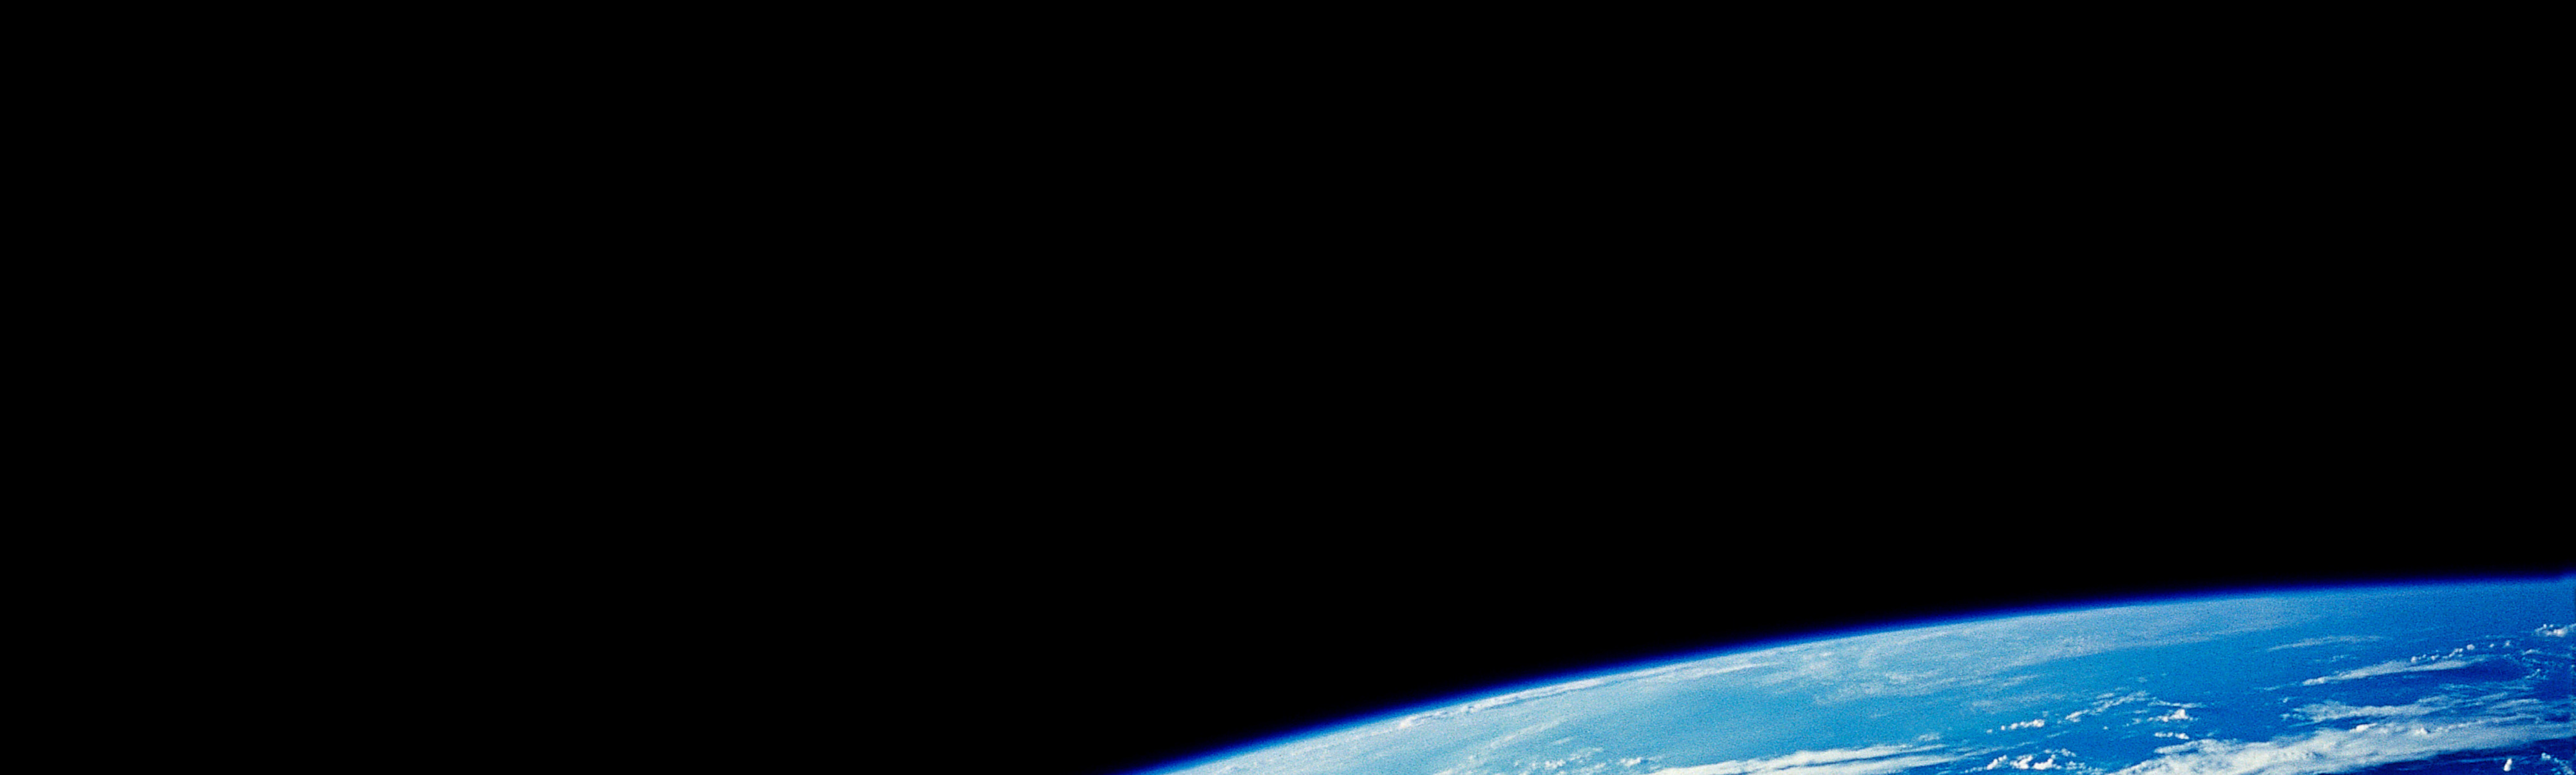
\includegraphics[width=\paperwidth]{figure/earth}}

\begin{document}
\begin{frame}[t]
  % Top title area
  %_____________________________________________________________________________________________
  \color{white} 
  \vspace*{2cm}
  \begin{columns}
    \begin{column}[t]{.97\textwidth}
      {\bfseries\fontsize{88}{120}\selectfont \inserttitle}
      %{\fontsize{88}{120}\selectfont\kern2cm---\kern2cm\insertsubtitle}
    \end{column}
  \end{columns}

  \vspace*{2cm}
  \begin{columns}
    \begin{column}[t]{.25\textwidth}
      {\fontsize{30}{36}\selectfont\insertauthor\\[0.5cm]
        \fontsize{30}{36}\selectfont{\itshape\insertinstitute}\\
        \fontsize{24}{18}\selectfont\texttt{\contact}}
    \end{column}

    \begin{column}[t]{.7\textwidth}
      {\fontsize{30}{36}\selectfont\setlength{\parskip}{15pt}Where is currently being developed at the Norwegian Mapping Authority (Kartverket). The software is written in Python, which has proved very fruitful. The code is quick to write and the architecture is easily extendable
and maintainable, while at the same time taking advantage of well-tested libraries
like the SOFA and IERS packages. Where is an open source project.

\vspace*{-10cm}

\endinput
}
      \raisebox{-2cm}{\kern52.5cm\color{white}\tiny PHOTO: GETTY IMAGES}
    \end{column}  
  \end{columns}



  \vspace*{1.5cm}
  \begin{columns}
    % Content area
    %_____________________________________________________________________________________________
    \begin{column}[t]{.68\textwidth}
      \begin{block}{}%Signal-in-space range error computation in Where}
        \begin{multicols}{2}

          {\fontsize{21}{36}\setlength{\parskip}{16pt}{\large\bfseries Introduction}\\
%_____________________________________________________________________________________________
Signal-in-space range error (SISRE) describes the statistical uncertainty of the modeled pseudorange due to errors in the broadcast orbit and clock information~\cite{montenbruck2015b}. SISRE is related to errors based on the space and control segments. That means influencing factors like clock stability, satellite antenna variation, signal imperfection and predictability of orbital motion for the space segment, as well as orbit and clock determination performance, distribution of monitoring stations, and upload capacity of the control segment~(\cite{heng2012},~\cite{montenbruck2015b}).

The Norwegian Mapping Authority has established a tool for monitoring Galileo and GPS orbit performance with the implementation of SISRE analysis in the geodetic software package \textbf{Where}. \textbf{Where} determines the global 
averaged SISRE based on comparisons between broadcast and precise orbit and clock products. The precise products are assumed to represent the truth.
%averaged SISRE based on comparison between broadcast and precise orbit and clocks products (see Figure~\ref{fig:diff_prec_brdc}), whereby the precise products are assumed to be truth. 

%The methodology used for the SISRE analysis, the input data and the results will be described in the following.

%\begin{figure}
%     \setbeamercolor{caption name}{fg=white}
%     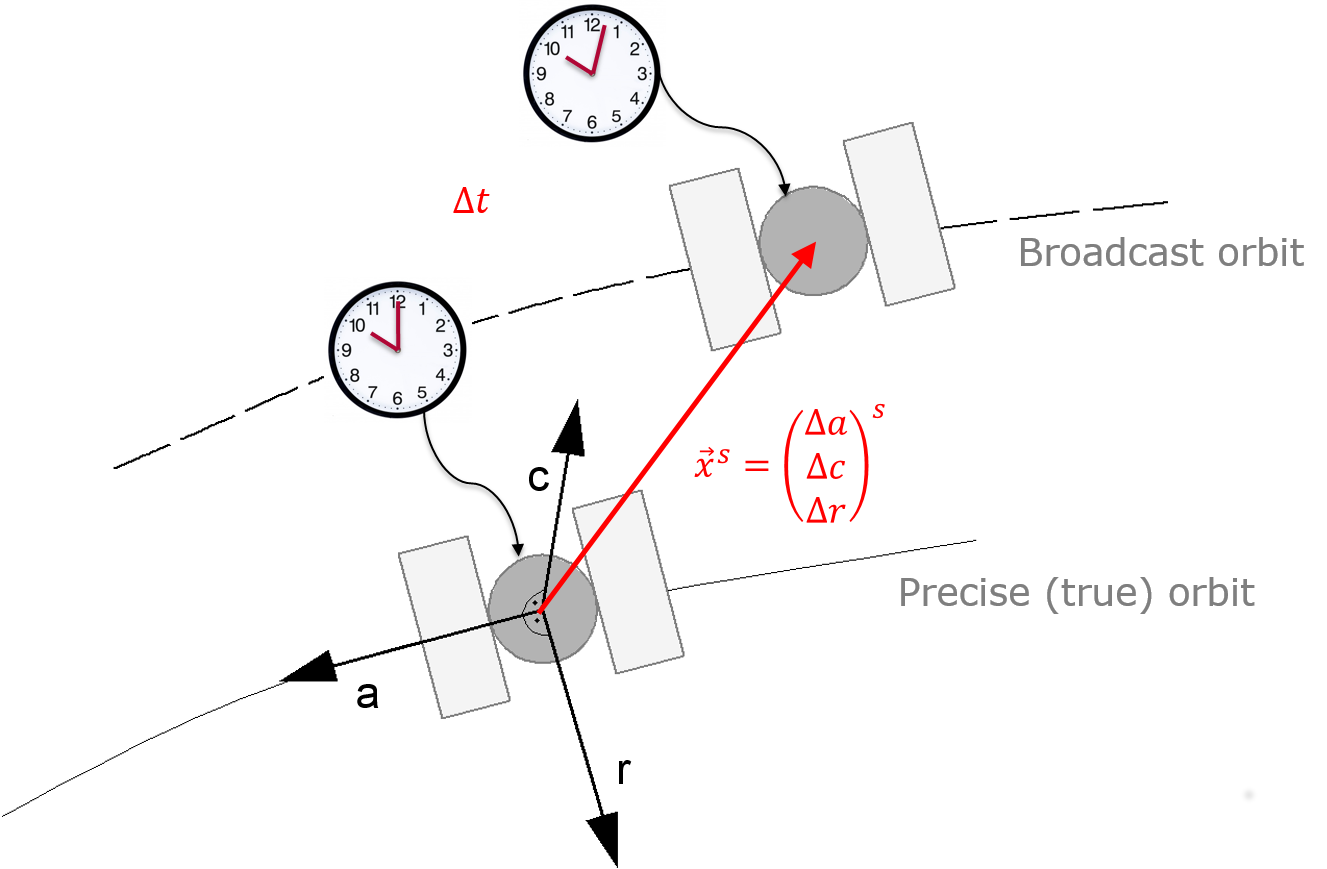
\includegraphics[width=0.3\textwidth]{figure/brdc_precise_comparison}
%     \caption{Satellite position given for precise (true) and broadcast orbit shown in local orbital reference frame (along-track, cross-track and radial) with orbit error vector $\vec x^s$. The elements of the orbit error vector are the differences between precise and broadcast orbits given in along-track $\Delta a$, cross-track $\Delta c$ and radial $\Delta r$ coordinates. In addition the difference between precise and broadcast satellite clock correction $\Delta t$ is illustrated. }
%    \label{fig:diff_prec_brdc}
%\end{figure}


{\large\bfseries Methodology}\\
%_____________________________________________________________________________________________
The SISRE analysis in \textbf{Where} is mainly based on Montenbruck et al.~\cite{montenbruck2018}, and will be presented in this section. 

Broadcast orbits and clocks refer to the satellite antenna phase center (APC). The precise orbits are related to the center-of-mass (CoM) and the precise clocks to the APC. The CoM is chosen as reference point in the SISRE analysis. That means the broadcast and precise orbits and clocks related to APC have to be transformed to the CoM by applying antenna phase center offsets (PCO). PCOs are given by the European GNSS Service Centre (GSC) and the International GNSS Service (IGS). The average of the GSC PCOs for E1/E5ab/E6 frequencies is used~\cite{montenbruck2018}.

Broadcast and precise clock products are referred to a specific conventional signal or signal combination, therefore a group delay correction has to be applied~\cite{montenbruck2018}. \textbf{Where} uses the IGS Multi-GNSS Experiment (MGEX) differential code bias product of the Chinese Academy of Sciences (CAS) for correcting precise clock products for the SISRE analysis of I/NAV navigation messages. 

For the SISRE analysis it is common to apply the average contribution over all points of the earth within the visibility cone of the satellite~\cite{montenbruck2015b}, which is called global averaged SISRE. The SISRE analysis in \textbf{Where} is based on the global averaged SISRE:

\begin{equation*}   
     \text{SISRE}^s(t) = \sqrt{(w_r \cdot \Delta r^s(t) - \Delta t^s(t))^2 + w_{a,c}^2 \cdot (\Delta {a^s}(t)^2 + \Delta {c^s}(t)^2)}
  \label{eq:sisre}  
\end{equation*}

with

\begin{center}
\begin{tabularx}{.9\columnwidth}{lX}
$\text{SISRE}^s$       & global averaged SISRE for satellite $s$, \\
$t$  & observation epoch, \\
$\Delta a^s$, $\Delta c^s$, $\Delta r^s$   & satellite coordinate differences between broadcast and precise ephemeris in local orbital reference frame with along-track, cross-track and radial coordinates, related to the CoM of satellite $s$,\\
$\Delta t^s$ & satellite clock correction difference related to CoM of satellite $s$ and corrected for satellite biases and averaged clock offset in each epoch,\\
$w_r$        & SISRE weight factor for radial errors, $w_r = 0.984$ is used for an elevation mask of $5^{\circ}$,\\
$w_{a,c}$    & SISRE weight factor for along-track and cross-track errors, $w_{a,c} = 0.124$ is used for an elevation mask of $5^{\circ}$.\\
\end{tabularx}
\end{center}

The SISRE analysis is carried out on daily basis. Each daily solution is cleaned for outliers. The outliers are detected and rejected iteratively for each day using a 4-sigma threshold determined for the complete Galileo satellite constellation. After each iteration the SISRE results are again recomputed.


\columnbreak
{\large\bfseries Input data and data preparation}\\
%_____________________________________________________________________________________________
Table~\ref{tab:data} gives an overview over the used input files and metadata in the SISRE analysis.

A sampling rate of 5 minutes is used in the SISRE analysis. %Therefore the precise orbit and clock data given for every 15 minutes and respectively 5 minutes has to be interpolated. A 9 degree Lagrange polynomial interpolation is applied for the precise orbits and a linear interpolation for the precise clocks.
The transmission time of navigation record is used for selection of the RINEX file navigation record based on a given observation time. It should be noted that \textbf{Where} sorts the navigation messages satellite-wise after time of transmission. Afterwards \textbf{Where} removes duplicated navigation messages for a satellite, keeping the first occurrence of the navigation message. The navigation record with the transmission time closest before a given observation epoch is chosen.
%\begin{equation*}   
%     min(t - t_{trans} \geq 0)
%  \label{eq:select_brdc}  
%\end{equation*}

A Galileo navigation data record is only valid for 4 hours after time of ephemeris and updated every 10 minutes to 3 hours as described in to Appendix C.4.4.1 in Galileo-OS-SDD~\cite{galileo-os-sdd}. Observation epochs are excluded if they exceed the validity length of the navigation record. In addition only healthy Galileo satellites are used in the analysis. 


{\large\bfseries Results}\\
%_____________________________________________________________________________________________
We have carried out a SISRE analysis with software package \textbf{Where} using data from January 1st until June 30th 2018. The results can be seen in the Figures~\ref{fig:sisre},~\ref{fig:sisre_stacked} and~\ref{fig:sisre_signal_comb} and Table~\ref{tab:sisre_results}.

Figure~\ref{fig:sisre} shows the global average SISRE results for all Galileo satellites for the signal combination E1/E5a using the F/NAV navigation message. The determined SISRE RMS is 17 cm for the half year time period and over all Galileo satellites. This is significantly better than for E1 and E1/E5b signal combination based on I/NAV message with 20 cm and 19 cm, respectively (see Table~\ref{tab:sisre_results}).

Figure~\ref{fig:sisre_stacked} illustrates the SISRE RMS for the Galileo satellites. The SISRE RMS solution is mostly driven by orbit errors. Clock and bias errors contributes only slightly to the complete SISRE solution. This can be explained by the fact that Galileo uses highly stable clocks and short update rates for the broadcast ephemeris~\cite{montenbruck2018}.

Figure~\ref{fig:sisre_signal_comb} represents the SIRSE 95th percentiles for single- and dual-frequency users on a monthly basis. Table~\ref{tab:sisre_results} shows the corresponding numbers for the complete half year period. The \textbf{Where} solution indicates differences up to few centimeters between the E1, E1/E5b and E1/E5a signal combinations, whereas the GSC solution based on the Galileo quarterly performance reports (\cite{galileo-is-os-2018-jan},~\cite{galileo-is-os-2018-apr}) does not show any significant differences. In addition the \textbf{Where} half year SISRE 95th percentiles are lower in comparison to GSC solution, especially with less than 10 cm for a E1/E5a user by applying F/NAV messages.


{\large\bfseries Summary}\\
%_____________________________________________________________________________________________
The first results of SISRE analysis with the software package \textbf{Where} are comparable to other studies (e.g.~\cite{galileo-is-os-2018-jan},~\cite{galileo-is-os-2018-apr} or~\cite{montenbruck2018}) with a global average SISRE RMS up to 20 cm and a monthly 95th percentile of 25\,-\,40 cm for the Galileo system. Further validation is needed to identify the cause of the differences seen between the \textbf{Where} and GSC solution. In addition the quality check of the input data has to be improved, which includes the used IGS broadcast, precise and DCB products. This is important to ensure the correct detection of Galileo system anomalies related to the control and satellite segment.

The Galileo SDD document~\cite{galileo-os-sdd} defines as minimum performance level, that 95\% SISRE over all healthy satellites and a period of 30 days should be less than 2 m. For the first half year in 2018 the Galileo system fulfills this minimum performance level for E1 single-frequency and for E1/E5b and E1/E5a dual-frequency users.

%\vspace*{15ex}

\endinput
}
          %{\large\bfseries Introduction}\\
%_____________________________________________________________________________________________
Signal-in-space range error (SISRE) describes the statistical uncertainty of the modeled pseudorange due to errors in the broadcast orbit and clock information~\cite{montenbruck2015b}. SISRE is related to errors based on the space and control segments. That means influencing factors like clock stability, satellite antenna variation, signal imperfection and predictability of orbital motion for the space segment, as well as orbit and clock determination performance, distribution of monitoring stations, and upload capacity of the control segment~(\cite{heng2012},~\cite{montenbruck2015b}).

The Norwegian Mapping Authority has established a tool for monitoring Galileo and GPS orbit performance with the implementation of SISRE analysis in the geodetic software package \textbf{Where}. \textbf{Where} determines the global 
averaged SISRE based on comparisons between broadcast and precise orbit and clock products. The precise products are assumed to represent the truth.
%averaged SISRE based on comparison between broadcast and precise orbit and clocks products (see Figure~\ref{fig:diff_prec_brdc}), whereby the precise products are assumed to be truth. 

%The methodology used for the SISRE analysis, the input data and the results will be described in the following.

%\begin{figure}
%     \setbeamercolor{caption name}{fg=white}
%     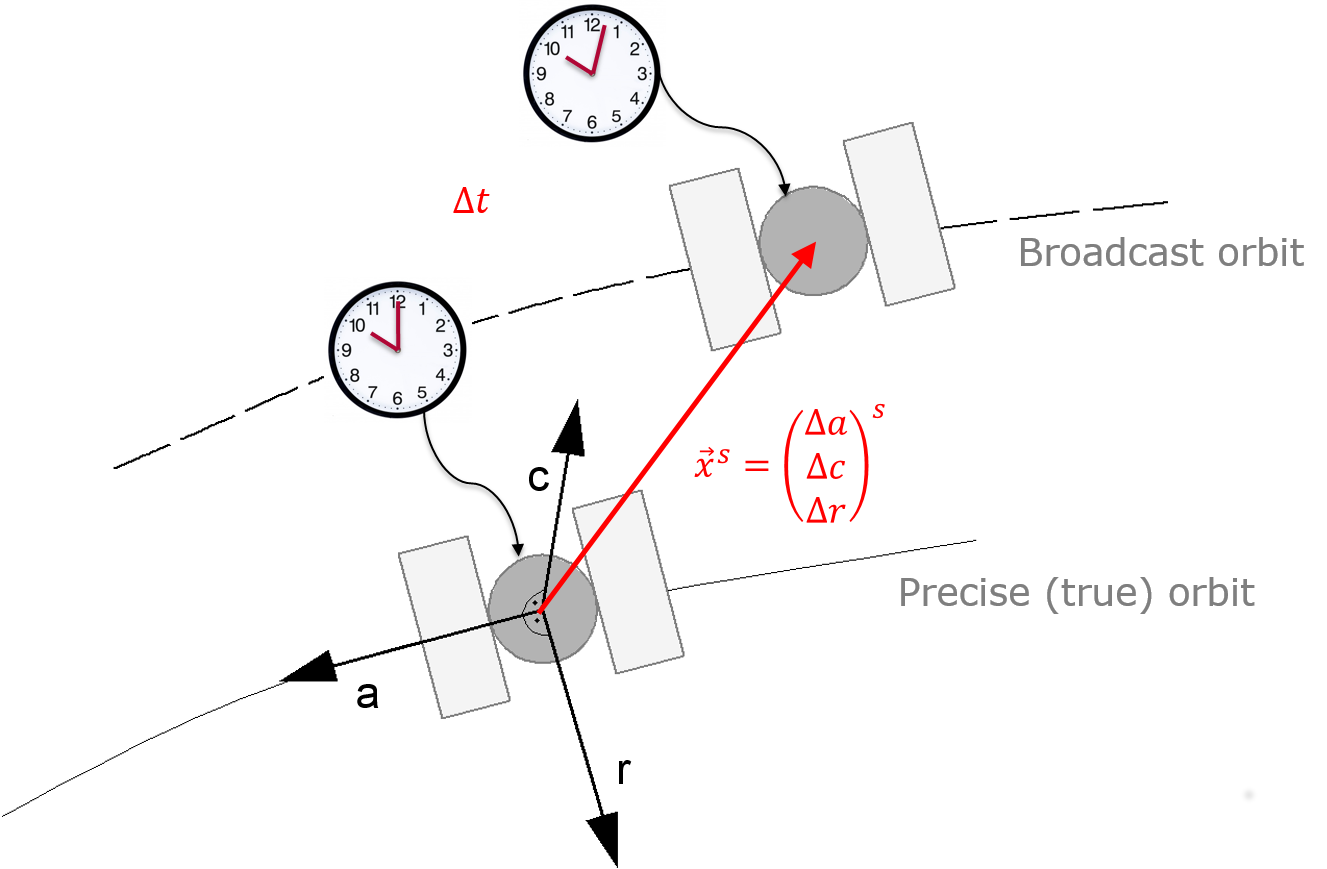
\includegraphics[width=0.3\textwidth]{figure/brdc_precise_comparison}
%     \caption{Satellite position given for precise (true) and broadcast orbit shown in local orbital reference frame (along-track, cross-track and radial) with orbit error vector $\vec x^s$. The elements of the orbit error vector are the differences between precise and broadcast orbits given in along-track $\Delta a$, cross-track $\Delta c$ and radial $\Delta r$ coordinates. In addition the difference between precise and broadcast satellite clock correction $\Delta t$ is illustrated. }
%    \label{fig:diff_prec_brdc}
%\end{figure}


{\large\bfseries Methodology}\\
%_____________________________________________________________________________________________
The SISRE analysis in \textbf{Where} is mainly based on Montenbruck et al.~\cite{montenbruck2018}, and will be presented in this section. 

Broadcast orbits and clocks refer to the satellite antenna phase center (APC). The precise orbits are related to the center-of-mass (CoM) and the precise clocks to the APC. The CoM is chosen as reference point in the SISRE analysis. That means the broadcast and precise orbits and clocks related to APC have to be transformed to the CoM by applying antenna phase center offsets (PCO). PCOs are given by the European GNSS Service Centre (GSC) and the International GNSS Service (IGS). The average of the GSC PCOs for E1/E5ab/E6 frequencies is used~\cite{montenbruck2018}.

Broadcast and precise clock products are referred to a specific conventional signal or signal combination, therefore a group delay correction has to be applied~\cite{montenbruck2018}. \textbf{Where} uses the IGS Multi-GNSS Experiment (MGEX) differential code bias product of the Chinese Academy of Sciences (CAS) for correcting precise clock products for the SISRE analysis of I/NAV navigation messages. 

For the SISRE analysis it is common to apply the average contribution over all points of the earth within the visibility cone of the satellite~\cite{montenbruck2015b}, which is called global averaged SISRE. The SISRE analysis in \textbf{Where} is based on the global averaged SISRE:

\begin{equation*}   
     \text{SISRE}^s(t) = \sqrt{(w_r \cdot \Delta r^s(t) - \Delta t^s(t))^2 + w_{a,c}^2 \cdot (\Delta {a^s}(t)^2 + \Delta {c^s}(t)^2)}
  \label{eq:sisre}  
\end{equation*}

with

\begin{center}
\begin{tabularx}{.9\columnwidth}{lX}
$\text{SISRE}^s$       & global averaged SISRE for satellite $s$, \\
$t$  & observation epoch, \\
$\Delta a^s$, $\Delta c^s$, $\Delta r^s$   & satellite coordinate differences between broadcast and precise ephemeris in local orbital reference frame with along-track, cross-track and radial coordinates, related to the CoM of satellite $s$,\\
$\Delta t^s$ & satellite clock correction difference related to CoM of satellite $s$ and corrected for satellite biases and averaged clock offset in each epoch,\\
$w_r$        & SISRE weight factor for radial errors, $w_r = 0.984$ is used for an elevation mask of $5^{\circ}$,\\
$w_{a,c}$    & SISRE weight factor for along-track and cross-track errors, $w_{a,c} = 0.124$ is used for an elevation mask of $5^{\circ}$.\\
\end{tabularx}
\end{center}

The SISRE analysis is carried out on daily basis. Each daily solution is cleaned for outliers. The outliers are detected and rejected iteratively for each day using a 4-sigma threshold determined for the complete Galileo satellite constellation. After each iteration the SISRE results are again recomputed.


\columnbreak
{\large\bfseries Input data and data preparation}\\
%_____________________________________________________________________________________________
Table~\ref{tab:data} gives an overview over the used input files and metadata in the SISRE analysis.

A sampling rate of 5 minutes is used in the SISRE analysis. %Therefore the precise orbit and clock data given for every 15 minutes and respectively 5 minutes has to be interpolated. A 9 degree Lagrange polynomial interpolation is applied for the precise orbits and a linear interpolation for the precise clocks.
The transmission time of navigation record is used for selection of the RINEX file navigation record based on a given observation time. It should be noted that \textbf{Where} sorts the navigation messages satellite-wise after time of transmission. Afterwards \textbf{Where} removes duplicated navigation messages for a satellite, keeping the first occurrence of the navigation message. The navigation record with the transmission time closest before a given observation epoch is chosen.
%\begin{equation*}   
%     min(t - t_{trans} \geq 0)
%  \label{eq:select_brdc}  
%\end{equation*}

A Galileo navigation data record is only valid for 4 hours after time of ephemeris and updated every 10 minutes to 3 hours as described in to Appendix C.4.4.1 in Galileo-OS-SDD~\cite{galileo-os-sdd}. Observation epochs are excluded if they exceed the validity length of the navigation record. In addition only healthy Galileo satellites are used in the analysis. 


{\large\bfseries Results}\\
%_____________________________________________________________________________________________
We have carried out a SISRE analysis with software package \textbf{Where} using data from January 1st until June 30th 2018. The results can be seen in the Figures~\ref{fig:sisre},~\ref{fig:sisre_stacked} and~\ref{fig:sisre_signal_comb} and Table~\ref{tab:sisre_results}.

Figure~\ref{fig:sisre} shows the global average SISRE results for all Galileo satellites for the signal combination E1/E5a using the F/NAV navigation message. The determined SISRE RMS is 17 cm for the half year time period and over all Galileo satellites. This is significantly better than for E1 and E1/E5b signal combination based on I/NAV message with 20 cm and 19 cm, respectively (see Table~\ref{tab:sisre_results}).

Figure~\ref{fig:sisre_stacked} illustrates the SISRE RMS for the Galileo satellites. The SISRE RMS solution is mostly driven by orbit errors. Clock and bias errors contributes only slightly to the complete SISRE solution. This can be explained by the fact that Galileo uses highly stable clocks and short update rates for the broadcast ephemeris~\cite{montenbruck2018}.

Figure~\ref{fig:sisre_signal_comb} represents the SIRSE 95th percentiles for single- and dual-frequency users on a monthly basis. Table~\ref{tab:sisre_results} shows the corresponding numbers for the complete half year period. The \textbf{Where} solution indicates differences up to few centimeters between the E1, E1/E5b and E1/E5a signal combinations, whereas the GSC solution based on the Galileo quarterly performance reports (\cite{galileo-is-os-2018-jan},~\cite{galileo-is-os-2018-apr}) does not show any significant differences. In addition the \textbf{Where} half year SISRE 95th percentiles are lower in comparison to GSC solution, especially with less than 10 cm for a E1/E5a user by applying F/NAV messages.


{\large\bfseries Summary}\\
%_____________________________________________________________________________________________
The first results of SISRE analysis with the software package \textbf{Where} are comparable to other studies (e.g.~\cite{galileo-is-os-2018-jan},~\cite{galileo-is-os-2018-apr} or~\cite{montenbruck2018}) with a global average SISRE RMS up to 20 cm and a monthly 95th percentile of 25\,-\,40 cm for the Galileo system. Further validation is needed to identify the cause of the differences seen between the \textbf{Where} and GSC solution. In addition the quality check of the input data has to be improved, which includes the used IGS broadcast, precise and DCB products. This is important to ensure the correct detection of Galileo system anomalies related to the control and satellite segment.

The Galileo SDD document~\cite{galileo-os-sdd} defines as minimum performance level, that 95\% SISRE over all healthy satellites and a period of 30 days should be less than 2 m. For the first half year in 2018 the Galileo system fulfills this minimum performance level for E1 single-frequency and for E1/E5b and E1/E5a dual-frequency users.

%\vspace*{15ex}

\endinput

        \end{multicols}
      \end{block}


      % Input data table strip
      %_____________________________________________________________________________________________
      \begin{alertblock}{}
           \begin{table}
              \color{black}
              \caption{Input data used for SISRE analysis.}
              \label{tab:data}
              \begin{tabular}{lll}
              \hline
              \rowcolor{kvgreen}\textcolor{white}{\textbf{Data}} & \textcolor{white}{\textbf{Institution  }} & \textcolor{white}{\textbf{URL}}\\
              \hline
              Broadcast orbit & DLR & ftp://cddis.gsfc.nasa.gov/gnss/data/campaign/mgex/daily/rinex3/\textit{yyyy}/\textit{ddd}/\textit{yy}p/brdm\textit{ddd}0.\textit{yy}p.Z\\
              Precise orbit & CODE & ftp://igs.ign.fr/pub/igs/products/mgex/\textit{wwww}/COD0MGXFIN\_\textit{yyyyddd}0000\_01D\_05M\_ORB.SP3.gz\\
              Precise clock & CODE & ftp://igs.ign.fr/pub/igs/products/mgex/\textit{wwww}/COD0MGXFIN\_\textit{yyyyddd}0000\_01D\_30S\_CLK.CLK.gz\\
              Antenna PCO (precise) & IGS & ftp://igs.org/pub/station/general/igs14.atx \\
              Antenna PCO (broadcast) & GSC & https://www.gsc-europa.eu/support-to-developers/galileo-satellite-metadata \\
                            
              Satellite bias & CAS & ftp://igs.ign.fr/pub/igs/products/mgex/dcb/\textit{yyyy}/CAS0MGXRAP\_\textit{yyyyddd}0000\_01D\_01D\_DCB.BSX.gz\\
              \hline
              \end{tabular}
           \end{table}
      \end{alertblock} 
    \end{column}

    % Figure strip
    %_____________________________________________________________________________________________
    \begin{column}[t]{.28\textwidth}

     \vspace*{1cm}
     \begin{figure}
       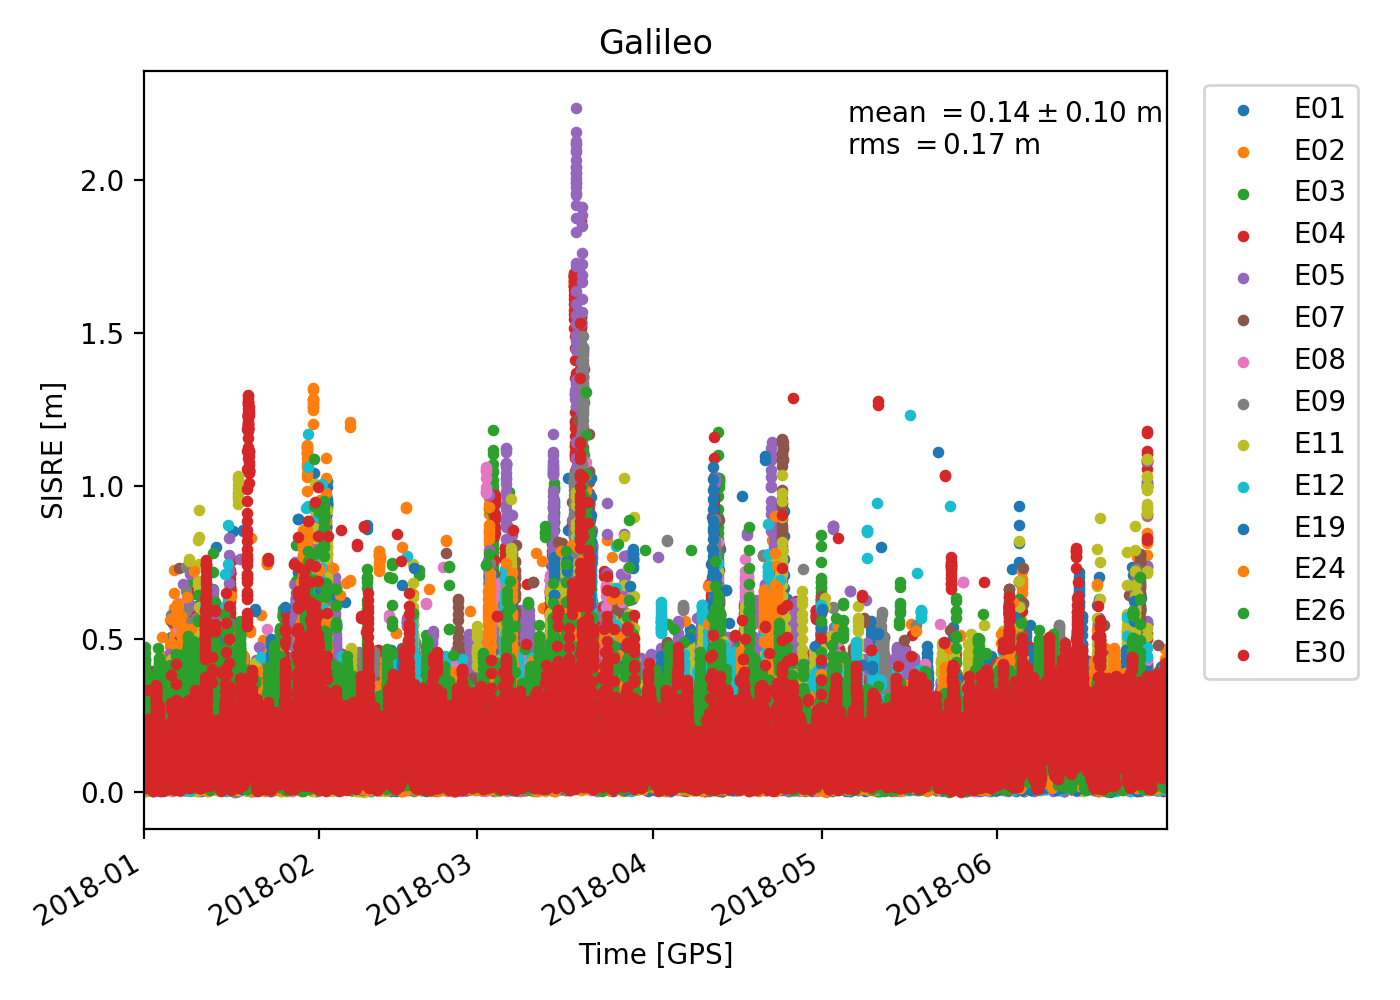
\includegraphics[width=\linewidth]{figure/plot_scatter_sisre_galileo}
       \caption{Global average SISRE for Galileo signal combination E1/E5a and use of F/NAV navigation message}
       \label{fig:sisre}
     \end{figure}

     \vspace*{1.5cm}

     \begin{figure}
       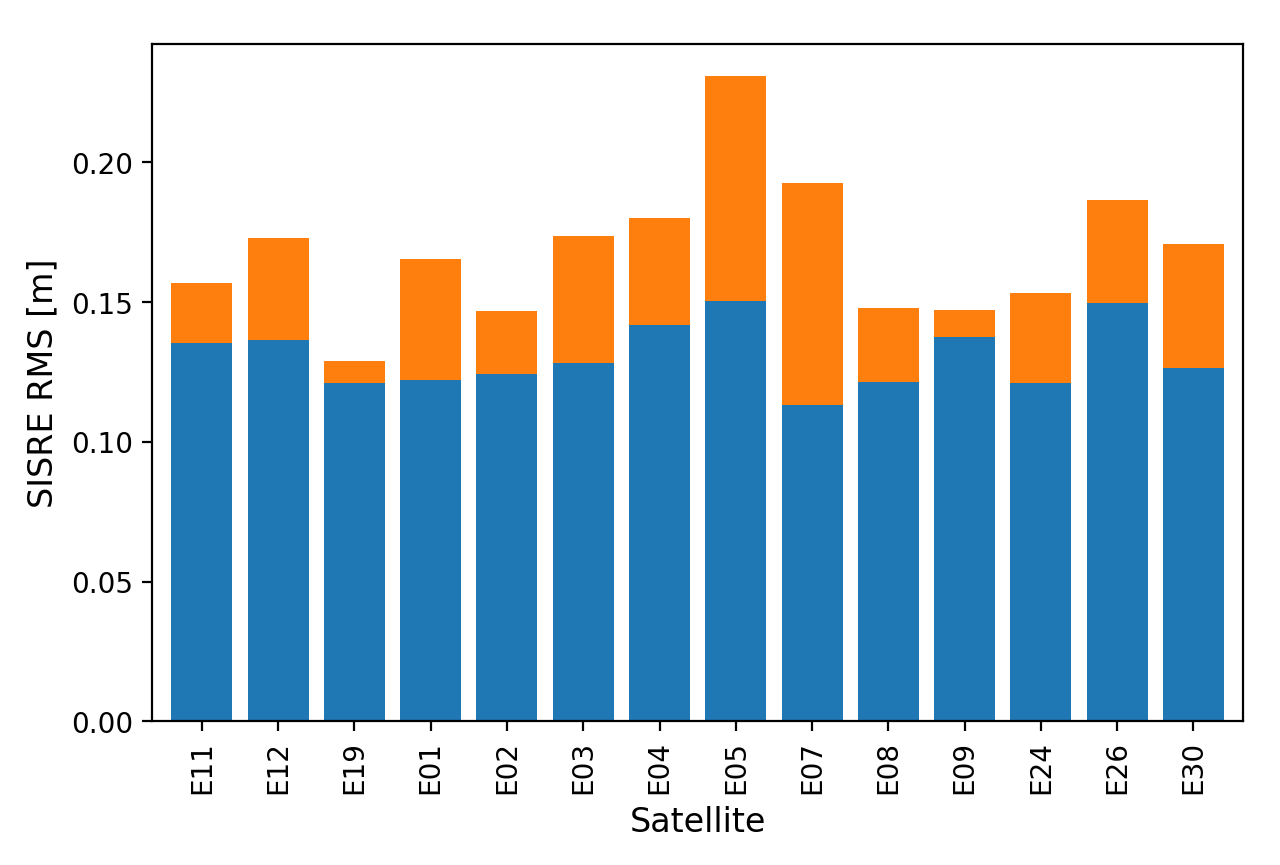
\includegraphics[width=\linewidth]{figure/plot_bar_stacked_sisre}
       \caption{SISRE RMS results of Galileo satellites for the period January 1st until June 30th 2018 and the signal combination E1/E5a with use of F/NAV navigation message. The sum of blue and orange bars illustrates the SISRE RMS, which includes orbit, clock and bias errors. The orbit-only SISRE RMS ($\Delta t^s = 0$ in SISRE equation) is represented by blue bars and includes only orbit errors.
}
       \label{fig:sisre_stacked}
     \end{figure}

     \vspace*{1.5cm}

     \begin{figure}
       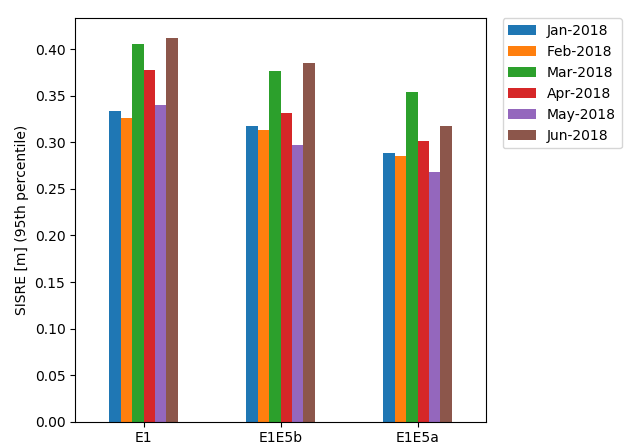
\includegraphics[width=\linewidth]{figure/plot_bar_sisre_signal_combination_percentile}
       \caption{Signal combination for Galileo single- and dual-frequency users, whereby E1 and E1/E5b users apply I/NAV and E1/E5a users F/NAV navigation message}
       \label{fig:sisre_signal_comb}
     \end{figure}

     \vspace*{1.5cm}

     \begin{table}
        \color{black}
        \caption{SISRE RMS and 95th percentile results for \textbf{Where} and GSC (\cite{galileo-is-os-2018-jan}, \cite{galileo-is-os-2018-apr}) solution are given for the complete Galileo satellite constellation and the period January 1st until June 30th 2018. The average is determined of the GSC monthly SISRE 95th percentiles given in \cite{galileo-is-os-2018-jan} and \cite{galileo-is-os-2018-apr}.}
        \label{tab:sisre_results}
        \begin{tabular}{lcccc}
        \hline
        \rowcolor{kvgreen}\textcolor{white}{\textbf{Signal}} & \textcolor{white}{\textbf{Nav. type}} & \textcolor{white}{\textbf{RMS}} & \textcolor{white}{\textbf{95th perc.}} & \textcolor{white}{\textbf{95th perc.}}\\
        \rowcolor{kvgreen}\textcolor{white}{} &  & \textcolor{white}{\textit{Where}} & \textcolor{white}{\textit{Where}} & \textcolor{white}{\textit{GSC}}\\
        \rowcolor{kvgreen}\textcolor{white}{} &  & \textcolor{white}{[cm]} & \textcolor{white}{[cm]} & \textcolor{white}{[cm]}\\

        \hline
        E1     & I/NAV & 20 & 38 & 41\\
        E1/E5b & I/NAV & 19 & 35 & 40\\
        E1/E5a & F/NAV & 17 & 31 & 41\\
        \hline
        \end{tabular}
     \end{table}


    \end{column}
   \end{columns}



  % References box
  \vspace*{1cm}
  \begin{columns}
    \begin{column}[t]{.15\textwidth}
      % Spacing (for Kartverket logo)
    \end{column}

    \begin{column}[t]{.82\textwidth}
      \begin{block}{}%References and Acknowledgements}
        \vspace*{-1cm}                   % Too much space on top inside block
        \begin{minipage}{.98\textwidth}  % Add space left and right
          \begin{multicols}{4}
            {\normalsize\bfseries References}\\
            \footnotesize
\bibliographystyle{../../where}
\bibliography{../../where}
\endinput

            \columnbreak

            {\normalsize\bfseries Acknowledgements}\\

            The authors would like to thank IGS for providing the needed input data and the Norwegian Space Centre for the financial support. A special thank to Peter Steigenberger (DLR) for his effort and patience answering our questions related to the SISRE analysis and be so kind to deliver SISRE test datasets. 
          \end{multicols}
        \end{minipage}
      \end{block}
    \end{column}
  \end{columns}
\end{frame}
\end{document}
